\section{Learning a prior on how things move}
We now describe our method for predicting dynamic 3D point clouds from pairs of images, and how we train it with our Stereo4D data.
Our model is based on \duster~\cite{wang2024dust3r}, which predicts a 3D point cloud for a static scene from images. Given two input images, it uses a ViT-based architecture~\cite{dosovitskiy2020image} to extract image features and uses a transformer-based decoder to cross-attend features from two images, and then use a downstream \textit{pointmap} decoder to output pointmaps for the two images, aligned in the first image's coordinate frame. 

\bfpar{\method model.}
While \duster focuses on static scene structure, our proposed \method method, illustrated in \Fig{method}, works with dynamic scenes by adding a \textit{motion} head that predicts how the points move between two frames. 
As input, \method accepts two images: $\mathbf{I}_0$ at time $t_0$, and $\mathbf{I}_1$ at time $t_1$ (where $t_0$ and $t_1$ may be seconds apart). 
It also accepts an intermediate query time $t_q \in [0,1]$; the motion head is asked to predict 3D scene flow from the two input frames to query time $t_q$, as described below.

Like \duster, \method begins by encoding the images with a shared ViT and cross-attention decoder, producing global features $G^0$ and $G^1$ for $\mathbf{I}_0$ and $\mathbf{I}_1$, respectively.
Each feature embedding can be converted into geometry using \duster's point head: e.g., for image $\mathbf{I}_0$, the point head produces a pointmap $\PB^0 \in \mathbb{R}^{H \times W \times 3}$ representing the geometry at time $t_0$, as well as a point confidence map $\CB^0_\mathsf{point} \in \mathbb{R}^{H \times W}$. 
Each point cloud is predicted in the coordinate frame of $\mathbf{I}_0$, but \emph{at the time of its respective image} (so, the two point clouds may differ due to scene motion).


We add a separate \textit{motion} head in parallel to the original point head, to predict a map of 3D displacement vectors (that is, a scene flow map, which we refer to as a \emph{motion map}) for each pointmap. 
The motion map should displace each input frame to an intermediate time $t_q \in [0,1]$, where $t_q = 0$ corresponds to $t_0$, the time of $\mathbf{I}_0$, and similarly for $t_q = 1$, $t_1$, and $\mathbf{I}_1$. The motivation for predicting motion to an intermediate time (inclusive of the endpoints) is twofold: first, it leads to a more general prediction task where we can predict a full motion trajectory between two frames, and second, it allows us to use partial ground truth 3D trajectories as supervision; not all trajectories may span all the way from $t_0$ to $t_1$, but may span through some intermediate time.

For each image $\IB_v$ (with $v \in \{0,1\}$), the network outputs a 3D motion map $\mathbf{M}^{v\to t_q}$ for the corresponding pointmap from $t_v$ to $t_q$ with corresponding motion confidence map $\CB_\mathsf{mot}^{v}\in\mathbb{R}^{H\times W}$. This prediction is based on the global feature $G^v$ as well as an embedding of the query time $\texttt{emb}(t_q)$. We use positional embedding~\cite{vaswani2017attention} to encode time $t_q$ to a 128-D vector and inject it to the motion features in the motion head via linear projection layers.

\bfpar{Training objective.} We use the same confidence-aware scale-invariant 3D regression loss
as in \duster. 
We first normalize both the predicted and ground truth pointmaps using scale factors $z=\text{norm}(\mathbf{P}^0, \mathbf{P}^1)$ and $\bar{z}=\text{norm}(\bar{\mathbf{P}}^0, \bar{\mathbf{P}}^1)$, respectively (where a bar, e.g., $\bar{\mathbf{P}}^0$, denotes a ground truth quantity, and where `$\text{norm}$' computes the average distance between a set of points and the world origin). 
We scale the motion maps with the same scales $z$ and $\bar{z}$. 
Following \duster, we compute a Euclidean distance loss on the pointmap, setting $\loss{point}$ to
{\small
\begin{equation}
    \sum_{v\in\{0,1\}}\sum_{i\in\mathcal{D}^v}\CB_{\mathsf{point},i}^v\left\|\frac{1}{z}\mathbf{P}_i^v - \frac{1}{\bar{z}}\bar{\mathbf{P}}_i^v\right\| - \alpha_p\log\CB_{\mathsf{point},i}^v
    \label{eqn:loss_point}
\end{equation}}
where $\mathcal{D}^v$ corresponds to the valid pixels where ground truth is defined and $\alpha_p$ is a weighting hyperparameter. 
We additionally compute a Euclidean distance loss on the position \emph{after motion}, which encourages the network to learn correct displacements. This loss $\loss{motion}$ is defined as
{\small
\begin{equation}\label{eqn:loss_motion}
    \sum_{v\in\{0,1\}}\sum_{i\in\mathcal{D}^v}\CB_{\mathsf{mot},i}^v\left\|\frac{1}{z}\mathbf{P}_i^{v\to t_q} - \frac{1}{\bar{z}}\bar{\mathbf{P}}_i^{v\to t_q}\right\| \\
    - \alpha_m\log\CB_{\mathsf{mot},i}^v,
\end{equation}}
where $ \mathbf{P}_i^{v\to t_q} = \mathbf{P}_i^v + \mathbf{M}_i^{v\to t_q}$.

 
\begin{figure}[t]
    \centering
    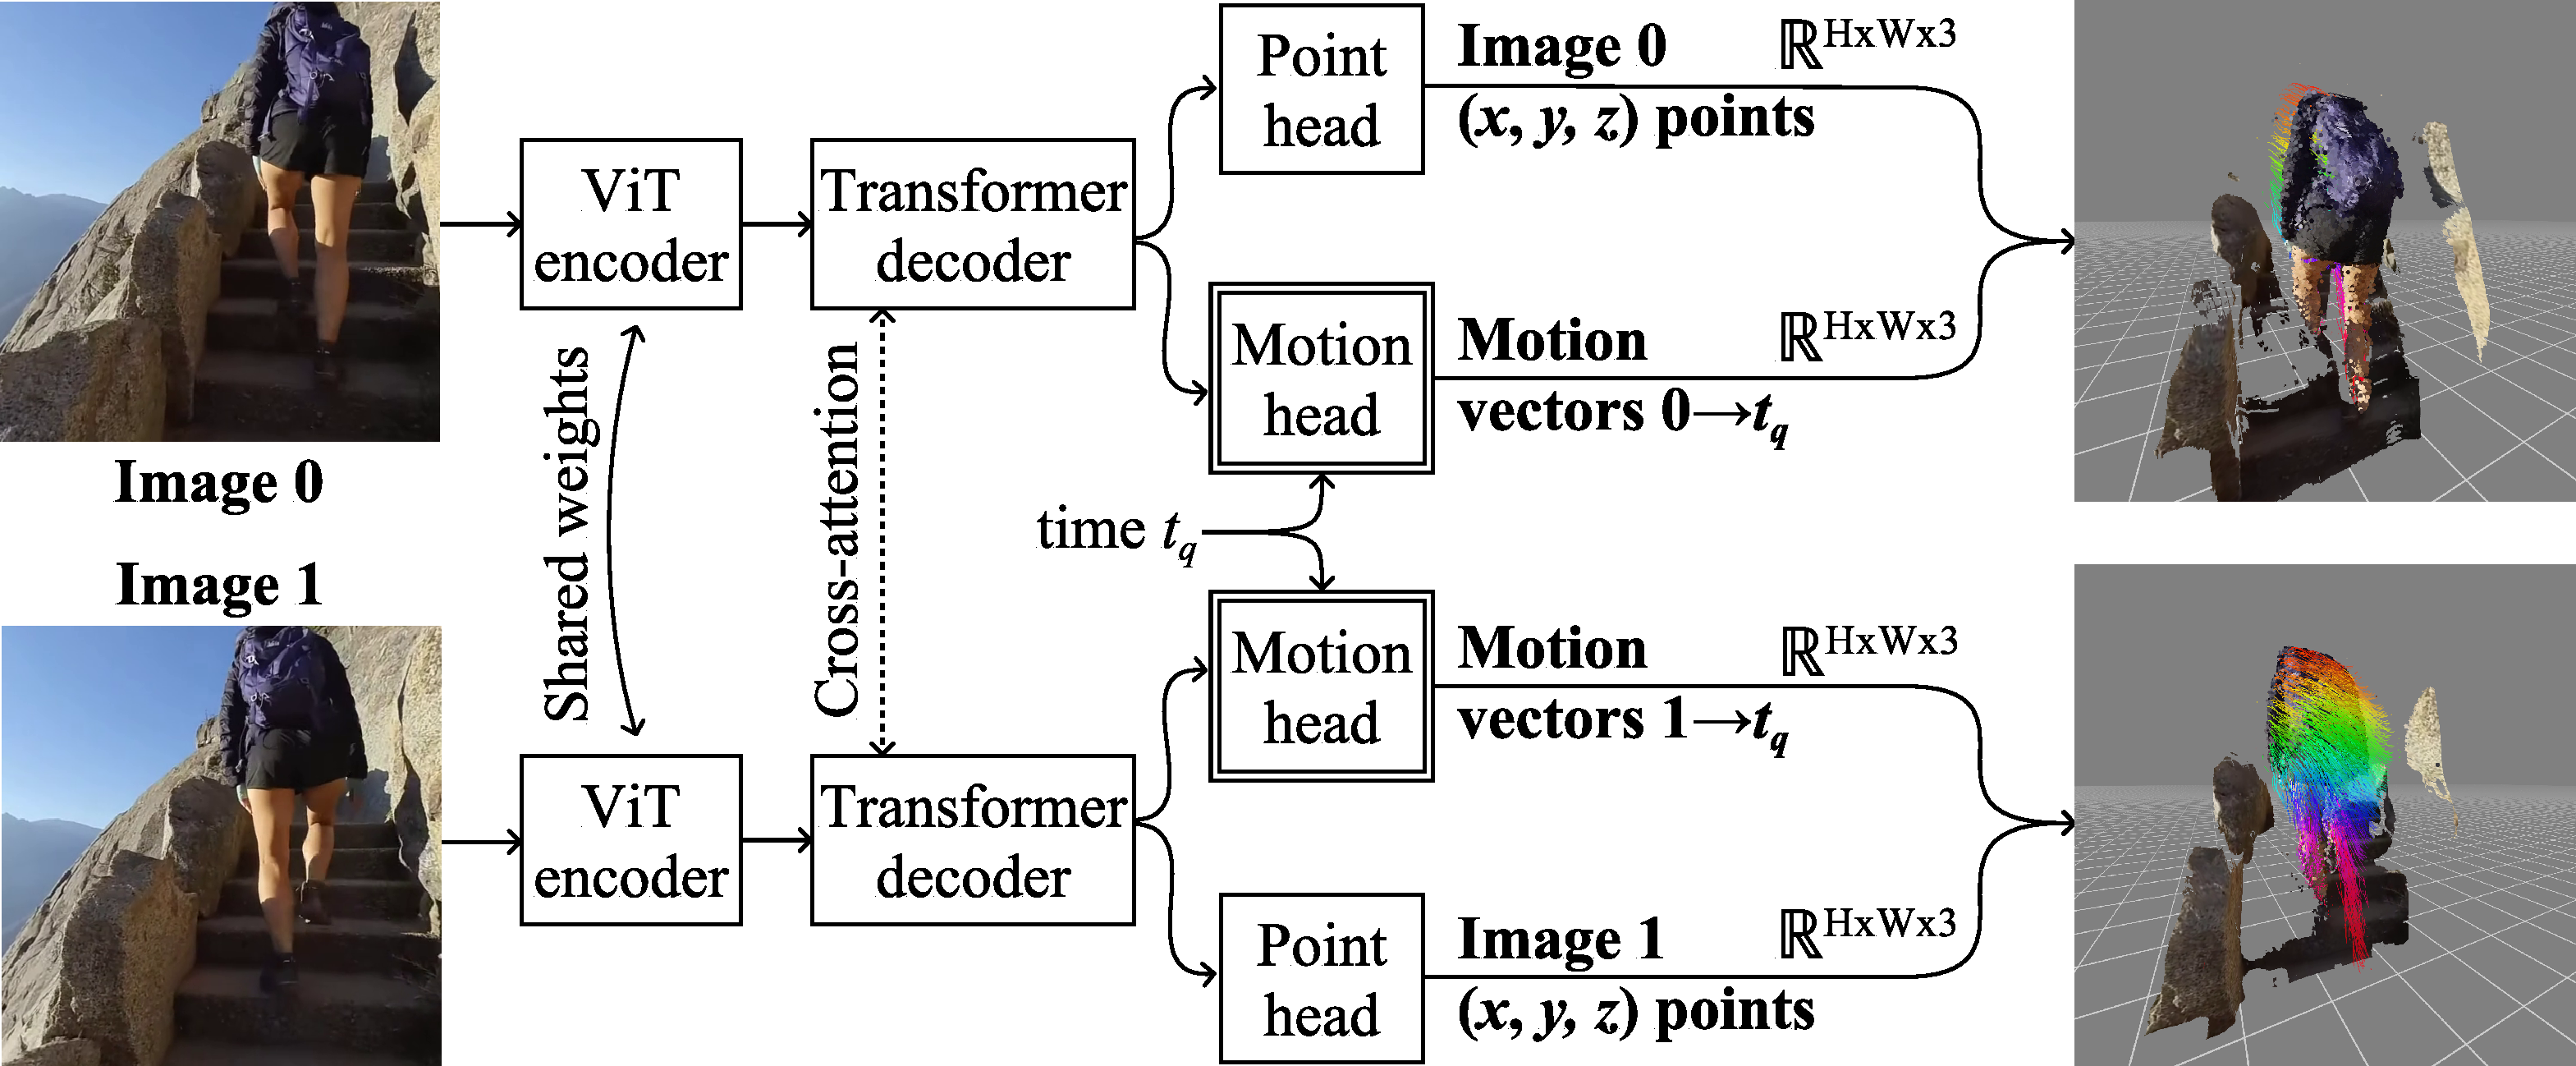
\includegraphics[width=\linewidth]{fig/method-HgkMYtMSdW4-clip8.pdf}
    \caption{\textbf{\method architecture.} Given two images $(\mathbf{I}_0, \mathbf{I}_1)$ of a dynamic scene and a desired target time $t_q$, the images are passed through a ViT encoder and transformer decoder. The resulting features are processed by (1) a pointmap head that predicts 3D points in the coordinate frame of $\mathbf{I}_0$, and (2) a 3D motion head that predicts the motion of all points to the target time $t_q$. A double outline indicates a new component compared to DUSt3R.}
    \label{fig:method}
\end{figure}

\bfpar{Training details.}
We initialize our network with \duster weights and initialize the motion head with the same weights as the point head. We finetune for 49k iterations, with batch size 64, learning rate 2.5e-5, optimized by Adam with weight decay 0.95. During training, we randomly sample pairs of video frames that are at most 60 frames apart. 
The weight for the confidence loss in Eqn~\ref{eqn:loss_point}-\ref{eqn:loss_motion} is $\alpha_m = \alpha_p = 0.2$. The model is trained on tracks extracted from both 60$^\circ$ FoV videos for (higher quality) and 120$^\circ$ FoV videos for (larger coverage). 
